\section{Физическая модель маятника}

Рассмотрим систему, состоящую из тележки массой $M$, движущейся по горизонтальной оси, и маятника с равномерно распределенной массой $m$ и длиной $l$,
закрепленного на шарнире на тележке. Примем за $x$ координату тележки, а за $\theta$ угол отклонения маятника от вертикали. Схема системы представлена на рисунке \ref{fig:pendulum}.
\begin{figure}[ht!]
    \centering
    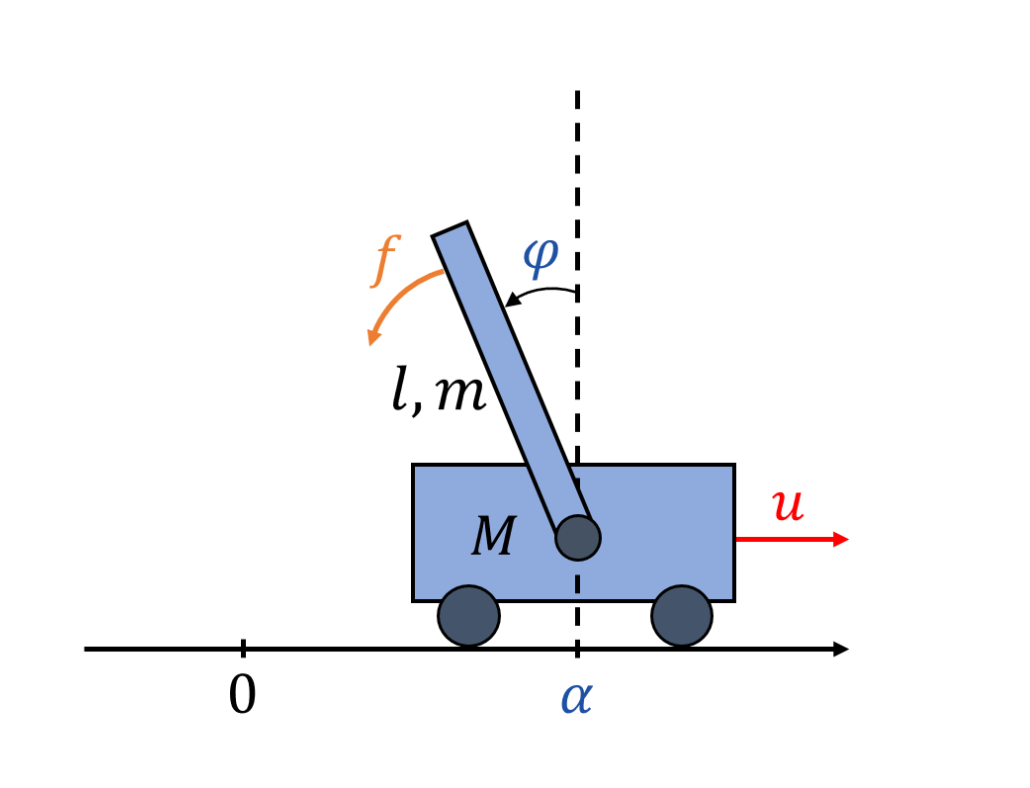
\includegraphics[width=0.5\textwidth]{media/cart.png}
    \caption{Схема маятника на тележке}
    \label{fig:pendulum}
\end{figure}

\subsection{Уравнения движения}
Используем законы Лагранжа для записи уравнений движения системы. 

Так как кинетическая и потенциальная зависят от центра масс тележки и маятника, введем в рассмотрение расстояние $l_{\text{com}}$ 
от точки подвеса маятника до его центра масс. При этом $l_{\text{com}} = \nicefrac{l}{2}$ для равномерно распределенной массы маятника.
В дальнейшем будем использовать $l$ для обозначения расстояния от точки подвеса до центра масс маятника. 

Напишем уравнения для координат центра масс маятника $x_m$ и $y_m$ и продифференцировав их по времени, получим скорости центра масс маятника:
\begin{equation}
    \begin{cases}
        x_m = x - l\sin\theta, \\
        y_m = l\cos\theta
    \end{cases} \Rightarrow
    \begin{cases}
        v_x = \dot{x} - l\dot{\theta}\cos\theta, \\
        v_y = -l\dot{\theta}\sin\theta
    \end{cases}
\end{equation}
Найдем квадрат скорости центра масс маятника $v_m$:
\begin{multline}
    v_m^2 = v_x^2 + v_y^2 = \left(\dot{x} - l\dot{\theta}\cos\theta\right)^2 + \left(-l\dot{\theta}\sin\theta\right)^2 \\
    \dot{x}^2 - 2l\dot{x}\dot{\theta}\cos\theta + l^2\dot{\theta}^2\cos^2\theta + l^2\dot{\theta}^2\sin^2\theta = \dot{x}^2 - 2l\dot{x}\dot{\theta}\cos\theta + l^2\dot{\theta}^2
\end{multline}
Общая энергия системы складывается из кинетической и потенциальной энергии маятника и кинетической энергии тележки:

Поступательная кинетическая энергия системы равна:
\begin{equation}
    T_m = \frac{1}{2}M\dot{x}^2 + \frac{1}{2}m v_m^2 =  \frac{1}{2} (M + m)\dot{x}^2 - m\dot{x}l\dot{\theta}\cos\theta + \frac{1}{2}ml^2\dot{\theta}^2
\end{equation}
Поскольку маятник вращается вокруг точки подвеса, его потенциальная энергия будет содержать 
вращательный компонент, который выражается через момент инерции маятника: 
\begin{equation}
    T_r = \frac{I\dot{\theta}^2}{2}
\end{equation}
\begin{equation}
    I = \frac{ml_{com}^2}{12} = \frac{ml^2}{3}
\end{equation}
Итого, полная кинетическая энергия системы равна: 
\begin{equation}
    T = \frac{1}{2} (M + m)\dot{x}^2 - m\dot{x}l\dot{\theta}\cos\theta + \frac{ml^2\dot{\theta}^2}{2} + \frac{ml^2\dot{\theta}^2}{6} 
\end{equation}  
Потенциальная энергия системы равна:
\begin{equation}
    U = mgl\cos\theta
\end{equation}
Записывая функция Лагранжа $L = T - U$, получаем: 
\begin{equation}
    L = \frac{1}{2} (M + m)\dot{x}^2 - m\dot{x}l\dot{\theta}\cos\theta + \frac{2ml^2\dot{\theta}^2}{3} - mgl\cos\theta
\end{equation}
Уравнения Лагранжа примут вид:
\begin{equation}
    \begin{array}{cc}
        \frac{d}{dt} \left( \frac{\partial L}{\partial \dot{x}} \right) - \frac{\partial L}{\partial x} = Q_x, \\
        \frac{d}{dt} \left( \frac{\partial L}{\partial \dot{\theta}} \right) - \frac{\partial L}{\partial \theta} = Q_{\theta}
    \end{array}
\end{equation}
где $Q_x$ и $Q_{\theta}$ -- обобщенные силы, действующие на тележку и маятник соответственно. В итоге получаем систему уравнений:
\begin{equation}
    \begin{cases}
        (M + m)\ddot{x} - ml\ddot{\theta}\cos\theta + ml\dot{\theta}^2\sin\theta = Q_x, \\
        \frac{4}{3} ml^2\ddot{\theta} - ml\ddot{x}\cos\theta - mgl\sin\theta = Q_{\theta}.
    \end{cases}
    \label{eq:forces_balance}
\end{equation}
Система уравнений \eqref{eq:forces_balance} представляет собой уравнения баланса сил, 
приложенных к тележке и моментов, действующих на маятник.

Запишем этм уравнения разрешив их относительно высших производных. Заметим, что вторые производные 
входят в эти уравнения линейно. С учетом этого приведем уравнения к матричному виду: 
\begin{equation}
    \begin{bmatrix}
        M + m &  -ml\cos\theta \\
        -ml\cos\theta & \frac{4}{3}ml^2 \\ 
    \end{bmatrix} \times
    \begin{bmatrix}
        \ddot{x} \\
        \ddot{\theta} \\
    \end{bmatrix} =
    \begin{bmatrix}
        -ml\dot{\theta}^2\sin\theta + Q_x \\ 
        mgl\sin\theta + Q_{\theta} \\
    \end{bmatrix}
\end{equation}
Убедимся в существовании и единственности решения системы:
\begin{equation}
    D = \frac{4}{3}ml^2(M + m) - m^2l^2\cos^2\theta = ml^2\left(\frac{4}{3}(M + m) - m\cos^2\theta\right) > 0
\end{equation}
Решая систему уравнений методом Крамера, получаем:
\begin{multline}
    \Delta_{\ddot{x}} = \begin{vmatrix}
        -ml\dot{\theta}^2\sin\theta + Q_x & -ml\cos\theta \\
        mgl\sin\theta + Q_{\theta} & \frac{4}{3}ml^2 \\
    \end{vmatrix} = \frac{4}{3}ml^2(-ml\dot{\theta}^2\sin\theta + Q_x) + ml\cos\theta(mgl\sin\theta + Q_{\theta}) 
\end{multline}
\begin{multline}
    \Delta_{\ddot{\theta}} = \begin{vmatrix}
        (M + m) & -ml\dot{\theta}^2\sin\theta + Q_x \\ 
        -ml\cos\theta & mgl\sin\theta + Q_{\theta} 
    \end{vmatrix} = (mgl\sin\theta + Q_{\theta})(M + m) + ml\cos\theta(-ml\dot{\theta}^2\sin\theta + Q_x) 
\end{multline}

В итоге получается систему дифференциальных уравнений, описывающих ускорение тележки и угловое ускорение маятника:
\begin{equation}
    \begin{cases}
        \ddot{x} = \frac{\frac{4}{3}ml^2(-ml\dot{\theta}^2\sin\theta + Q_x) + ml\cos\theta(mgl\sin\theta + Q_{\theta}) }{ml^2(\frac{4}{3}(M + m) - m\cos^2\theta)} \\ 
        \ddot{\theta} = \frac{(mgl\sin\theta + Q_{\theta})(M + m) + ml\cos\theta(-ml\dot{\theta}^2\sin\theta + Q_x) }{ml^2(\frac{4}{3}(M + m) - m\cos^2\theta)} \\ 
    \end{cases}
    \label{eq:nonlinear_model}
\end{equation}

Можно записать систему в пространстве состояний $X$ в форме Коши: 
\begin{equation}
    \begin{array}{cc}
        X = \begin{bmatrix} 
            x \\
            \dot{x} \\
            \theta \\
            \dot{\theta}
    \end{bmatrix} & 
    \dot{X} = \begin{bmatrix}
        \dot{x} \\
        \frac{\frac{4}{3}ml^2(-ml\dot{\theta}^2\sin\theta + Q_x) + ml\cos\theta(mgl\sin\theta + Q_{\theta})}{ml^2(\frac{4}{3}(M + m) - m\cos^2\theta)} \\ 
        \dot{\theta} \\
        \frac{(mgl\sin\theta + Q_{\theta})(M + m) + ml\cos\theta(-ml\dot{\theta}^2\sin\theta + Q_x) }{ml^2(\frac{4}{3}(M + m) - m\cos^2\theta)} \\ 
    \end{bmatrix}
    \end{array}
\end{equation}
где $X$ -- вектор состояния системы, состоящий координаты тележки $x$, скорости тележки $\dot{x}$, угла отклонения маятника от вертикали $\theta$ и угловой скорости маятника $\dot{\theta}$. 

Измеряемым выходом системы будет считать вектор $Y$, состоящий из координат тележки и угла отклонения маятника от вертикали:
\begin{equation}
    Y = \begin{bmatrix}
        1 & 0 & 0 & 0 \\
        0 & 0 & 1 & 0 \\ 
    \end{bmatrix} X
\end{equation}

\subsection{Точки равновесия}
Найдем точки равновесия системы в отсутствие внешних сил ($Q_x = Q_{\theta} = 0$). 
Для этого приравняем к нулю правые части уравнений движения, решим систему уравнений:
\begin{equation}
    \dot{X} = 0 \Rightarrow 
    \begin{cases}
        \dot{x} = 0, \\
        \dot{\theta} = 0, \\
        \frac{\frac{4}{3}ml^2(-ml\dot{\theta}^2\sin\theta + Q_x) + ml\cos\theta(mgl\sin\theta + Q_{\theta}) }{ml^2(\frac{4}{3}(M + m) - m\cos^2\theta)} = 0 \\
        \frac{(mgl\sin\theta + Q_{\theta})(M + m) + ml\cos\theta(-ml\dot{\theta}^2\sin\theta + Q_x) }{ml^2(\frac{4}{3}(M + m) - m\cos^2\theta)}  = 0 \\ 
    \end{cases}
\end{equation}
Упростив, получаем: 
\begin{equation}
    \begin{cases}
        \sin\theta(g(M + m) + ml\cos\theta) = 0 \\ 
        \sin\theta(ml + g\cos\theta) = 0
    \end{cases}
\end{equation}
Решая систему уравнений, получаем:
\begin{equation}
    \sin\theta = 0 \quad\Rightarrow\quad \theta = \pi n, n \in Z
\end{equation}
Существует бесконечное множество точек на окружности, которые соответствуют равновесию системы, будем рассматривать толко 
точки в пределах $[0, 2\pi]$, что соответствует одному \textit{обороту} маятника.
Таким образом, точки равновесия системы определяются углом отклонения маятника от вертикали $\theta = 0$ и $\theta = \pi$, 
что соответствует наивысшему и наинизшему положению маятника соответственно, что сходится с ожидаемым результатом. 

\subsection{Линейная модель}
Для дальнейшего анализа системы ее необходимо линеаризовать. Линеаризацию необходимо проводить в точках равновесия 
системы, которые были найдены в предыдущем пункте, в противном случае отклонения линейной модели от реальной системы будут велики. 
Линеаризуем систему в точке равновесия $\theta = 0$ и $x = 0$, используя то, что $\sin x \approx x$, $\cos x \approx 1$, $x^{n + 1} \approx 0, n \in N$ 
при малых $x$. 

\begin{equation}
    \dot{X} = \begin{bmatrix}
        \dot{x} \\
        \frac{4l Q_x + 3(mgl\theta + Q_{\theta})}{l(4M + m)} \\ 
        \dot{\theta} \\
        \frac{3(g\theta + \frac{Q_{\theta}}{ml})(M + m) + 3Q_x }{l(4M + m)} \\ 
    \end{bmatrix}
\end{equation}
% \begin{equation}
%     \dot{X} = \begin{bmatrix}
%         \dot{x} \\
%         \frac{lQ_x + mgl\theta + Q_{\theta} }{lM} \\ 
%         \dot{\theta} \\
%         \frac{(g\theta + \frac{Q_{\theta}}{ml})(M + m) + Q_x}{lM} \\ 
%     \end{bmatrix}
% \end{equation}

Запишем систему в матричном виде, принимая за управление обобщенную силу, приложенную на каретку, а за внешнее 
внешнее возмущение обобщенную силу, приложенную на маятник $u = Q_x, f = Q_{\theta}$:
\begin{equation}
    \begin{cases}
        \dot{x} = Ax + Bu + Df \\ 
        y = Cx
    \end{cases}
    \label{eq:linear_model}
\end{equation}
\begin{equation}
    \begin{array}{cc}
        \begin{bmatrix}
        \dot{x} \\
        \ddot{x} \\
        \dot{\theta} \\
        \ddot{\theta} \\
    \end{bmatrix} = \begin{bmatrix}
        0 & 1 & 0 & 0 \\
        0 & 0 & \frac{3mg}{4M + m} & 0 \\
        0 & 0 & 0 & 1 \\
        0 & 0 & \frac{3g(M + m)}{l(4M + m)} & 0 \\
    \end{bmatrix} \times \begin{bmatrix}
        x \\
        \dot{x} \\
        \theta \\
        \dot{\theta} \\
    \end{bmatrix} + \begin{bmatrix}
        0 \\
        \frac{4}{4M + m} \\
        0 \\
        \frac{3}{l(4M + m)} \\
    \end{bmatrix} \times Q_x + \begin{bmatrix}
        0 \\
        \frac{3}{l(4M + m)} \\
        0 \\
        \frac{3(M + m)}{ml^2(4M + m)} \\ 
    \end{bmatrix} \times Q_{\theta}  \\[4em]
    y = \begin{bmatrix}
        1 & 0 & 0 & 0 \\
        0 & 0 & 1 & 0 \\ 
    \end{bmatrix} \times \begin{bmatrix}
        x \\
        \dot{x} \\
        \theta \\
        \dot{\theta} \\
    \end{bmatrix}
    \end{array}
\end{equation}
Таким образом, матрицы системы примут вид: 
\begin{equation}
    A = \begin{bmatrix}
        0 & 1 & 0 & 0 \\
        0 & 0 & \frac{3mg}{4M + m} & 0 \\
        0 & 0 & 0 & 1 \\
        0 & 0 & \frac{3g(M + m)}{l(4M + m)} & 0 \\
    \end{bmatrix}, B = \begin{bmatrix}
        0 \\
        \frac{4}{4M + m} \\
        0 \\
        \frac{3}{l(4M + m)} \\
    \end{bmatrix}, D = \begin{bmatrix}
        0 \\
        \frac{3}{l(4M + m)} \\
        0 \\
        \frac{3(M + m)}{ml^2(4M + m)} \\
    \end{bmatrix}, C = \begin{bmatrix}
        1 & 0 & 0 & 0 \\
        0 & 0 & 1 & 0 \\ 
    \end{bmatrix}
\end{equation}
